\chapter{Application}
\label{chap:application}
The GNN model introduced in \autoref{chap:gnn} will be benchmarked on various datasets in the following chapters. All reference data was calculated using the 6-31G(2df,p) basis at theory level B3LYP. \\

Models will be evaluated by their iteration count till convergence, the energy difference from the converged solution and the RMSE of the diis commutator norm. 

\TODO{Refer to 0d benchmark model, check basis + functional}
\section{QM9 - \ch{C7H10O2} Isomers}
\label{sec:qm9_isomers_benchmark}
There are 6095 structural isomers of \ch{C7H10O2} in the QM9 dataset (see \autoref{subsec:qm9}). Analogous to the trials performed in \autoref{sec:further_trials_mlp}, we will train and validate on a randomly drawn sample of 500 isomers\footnote{using \texttt{scf\_guess\_datasets} (see \autoref{subsec:gnn_normalization})}. This reduction is necessary to make training and hyperparameter-tuning feasible in the scope of the thesis. Contrary to the full matrix prediction schemes in \autoref{chap:fock_matrix_predictions}, we employ sub-matrix predictions and reconstruct the full matrix thus making the actual number of samples significantly higher. Per molecule sample we get 7, 10 and 2 samples for \ch{C}, \ch{H} and \ch{O} respectively, totalling 3500 \ch{C}, 5000 \ch{H} and 1000 \ch{O} samples. This already provides some rotational variability. Additional rotations can be introduced through data augmentation during training to develop a model that is agnostic to rotation when predicting density.\\

\subsection{Initial training}
\label{subsec:qm9_isomers_initial}
To gauge the performance of the GNN devised in \autoref{chap:gnn} manual runs were performed during development. Hyperparameters were set according to \autoref{tab:init_hparams}. 

\begin{table}[H]
    \centering
    \caption{Hyperparameters used for the initial MGNN training (manually selected)}
    \label{tab:init_hparams}
    \begin{tabular}{ll ll}
        \toprule
        \textbf{Hyperparameter} & \textbf{Value} & \textbf{Hyperparameter} & \textbf{Value} \\
        \midrule
        Hidden dimension & 256 & Msg. passing rounds & 4 \\
        MsgNet layers & 3 & MsgNet dropout & 15 \% \\
        Batch size & 16 & Grace period & 10 epochs \\
        Target & Density matrix & Loss function & MSE (block-wise) \\
        Learn rate (initial) & $2.68 \times 10^{-3}$ & Weight decay & $1.78 \times 10^{-5}$ \\
        Optimizer & AdamW & Data augmentation & No \\
        \midrule
        Learn rate factor & 0.5 & Learn rate patience & 3 epochs \\
        Learn rate threshold & $10^{-3}$ & Learn rate cooldown & 2 epochs \\
        Learn rate min & $10^{-6}$ & — & — \\
        \bottomrule
    \end{tabular}
\end{table}
Note, that this initial run did not use data augmentation and thus trained on 400 samples (corresponding to our default datasplit of 80\% / 10\% / 10\%). The grace period, time without improvement, was set to 10 epochs to allow the learning rate scheduler sufficient time to take effect and for potential improvements to manifest thereafter.\\
Training and validation losses both monotonically decrease up to around epoch 30 as can be seen in \autoref{fig:initial_train_qm9_isomers}. While the loss on the validation set plateaus rather early, training loss decreases throughout the training process. 

\begin{figure}[H]
    \centering
    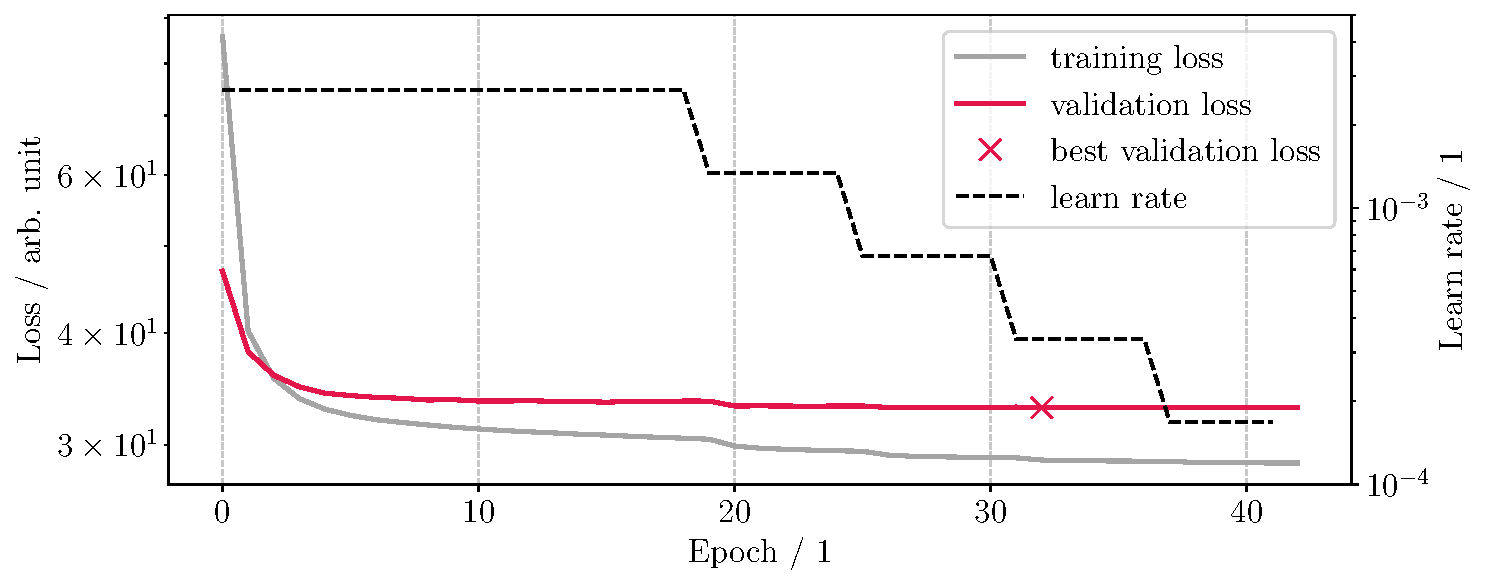
\includegraphics[width=\textwidth]{../fig/gnn/MGNN_6-31G_NO_AUG_07_07_manual_ref_train_val_loss.pdf}
    \caption[Initial GNN loss on QM9-isomers]{Initial GNN training / validation loss and corresponding learn rate per epoch on QM9-isomers.}
    \label{fig:initial_train_qm9_isomers}
\end{figure}
Both losses are further pushed down following learn rate decreases. This run produced the best model in epoch 33 with a validation loss of $33.00$ and a training loss of $28.83$ indicating slight overfitting which is to be expected especially without data augmentation in the training samples. The performance of the model $\text{GNN}_\text{initial}$ on the test set is compared to other models and guessing schemes in \autoref{tab:qm9_isomers_test_overview}. 
\TODO{Define DIIS RMSE}


\subsection{Hyperparameter tuning}
\label{subsec:qm9_isomers_hyperparamtuning}

\TODO{Investigate edge\_threshold}


Run 03/07
\begin{verbatim}
    Best hyperparameters found were:  {'batch_size': 32, 
    'hidden_dim': 128, 'message_passing_steps': 4, 'edge_threshold_val': 3.048869727327686, 
    'message_net_dropout': 0.2216763962125841, 'data_aug_factor': 1.0, 'message_net_layers': 3, 
    'lr': 0.0026826922264871233, 'weight_decay': 1.7769044544789348e-05, 'num_epochs': 30, 
    'grace_epochs': 5, 'lr_factor': 0.5, 'lr_patience': 3, 'lr_threshold': 0.001, 'lr_cooldown': 2, 
    'lr_min': 1e-06}
    Results saved to /home/ewachmann/REPOS/Masterarbeit/3_studies/Block_guessing/6-31g_testing/tune_results/results_hyp_small.py_20250703_123357.json 
    and best result to /home/ewachmann/REPOS/Masterarbeit/3_studies/Block_guessing/6-31g_testing/tune_results/best_hyp_small.py_20250703_123357.json
    Ray Tune run completed successfully.
\end{verbatim}


\subsection{Evaluation \& Conclusion}
\label{subsec:qm9_isomers_eval_and_concl}
The models defined above are compared to PySCF guessing schemes in \autoref{tab:qm9_isomers_test_overview}
\begin{table}[H]
    \centering
    \caption{Comparison of different models with PySCF guessing schemes.}
    \label{tab:qm9_isomers_test_overview}
    \begin{tabular}{l
                    S[table-format=2.1(2)]
                    S[table-format=-4(4)]
                    S[table-format=-1.3(2)]
                    S[table-format=2.1(1.1)]}
        \toprule
        Mean metrics:                 & {Iterations / 1} & {$\Delta E_\text{HF}$ / $\unit{\hartree}$}  & {$\delta E_\text{HF}$ / 1} & {DIIS error / $\unit{\hartree}$} \\
        \midrule
        $\text{GNN}_\text{initial}$   & 11.2(5)  & 9000(9300)  & 5.8(60)   & 0.17(2)  \\
        $\text{GNN}_\text{hyp. best}$ &          &             &           &          \\
        0-D                           & 17.1(15) & -26(13)     & -0.017(8) & 0.01(0)  \\
        1-e                           & 18.8(18) & -8000(100)  & -5.087(13)& 0.51(6)  \\
        vsap                          & 14.2(9)  & -8500(4)    & -5.45(5)  & 1.15(10) \\
        atom                          & 16.6(19) & -8600(30)   & -5.51(6)  & 1.12(10) \\
        minao                         & 10.8(6)  & -8122(3)    & -5.21(4)  & 2.0(3)   \\
        \bottomrule
    \end{tabular}
\end{table}

\section{QM9 - full?}
\label{sec:qm9_isomers_benchmark}
\TODO{Notes on training}

\section{MD ? }
\label{sec:qm9_isomers_benchmark}
\TODO{Notes on training}
